\documentclass{article}
\usepackage[left=2cm,right=2cm,top=2cm,bottom=2cm]{geometry}
\usepackage[utf8]{inputenc}
\usepackage[german]{babel}
\usepackage{amsmath}
\usepackage{dsfont}
\usepackage[export]{adjustbox}
\usepackage{amsthm}
\usepackage{color}
\usepackage{amsfonts}
\usepackage{amssymb}
\usepackage{wasysym}
\usepackage{makeidx}
\usepackage{graphicx}
\usepackage[colorlinks=true,urlcolor=blue,linkcolor=blue]{hyperref}
\usepackage{ziffer}
\usepackage{minted}
\usepackage{xcolor}
\usepackage{framed}
\usepackage{mdframed}
\usepackage{subfiles}
\usemintedstyle{emacs}

\definecolor{purp}{HTML}{9A72AC}
\definecolor{re}{HTML}{FC6255}
\definecolor{gre}{HTML}{83C167}
\definecolor{blu}{HTML}{58C4DD}
\definecolor{shadecolor}{rgb}{0.85,0.85,0.85}
\definecolor{bg}{rgb}{0.95,0.95,0.95}
\setlength{\parindent}{0em} 

\BeforeBeginEnvironment{minted}{\begin{mdframed}[linewidth =2 ,backgroundcolor=bg , linecolor=black, linewidth=0.5]}
\AfterEndEnvironment{minted}{\end{mdframed}}

\newtheorem{defi}{Definition}
\BeforeBeginEnvironment{defi}{\begin{mdframed}[linewidth =2 ,backgroundcolor=bg , linecolor=black, linewidth=0.5]}
\AfterEndEnvironment{defi}{\end{mdframed}}

\newcommand{\bsp}{\textbf{Beispiel}:}
%\newcommand{\task}{\textbf{Aufgabe}:}

\newcommand{\bol}[1]{\textbf{#1}}
\newcommand{\q}[1]{\glqq #1\grqq}
\newcommand{\DODO}[1]{\textbf{\textcolor{red}{DODO:}} #1 \\ \begin{center}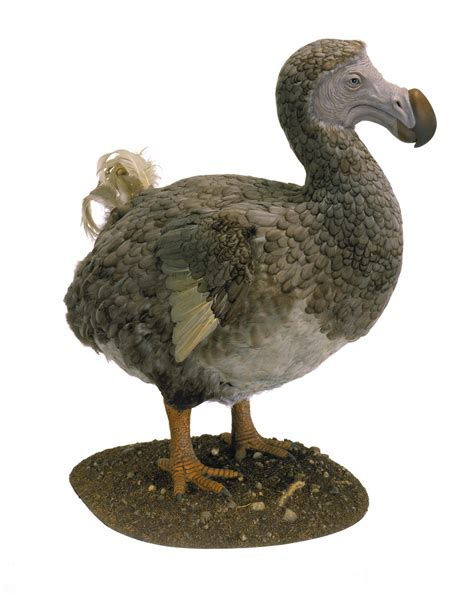
\includegraphics[scale=0.2]{../../media/dodo.jpg} \end{center}}

\newenvironment{task}[1]{
    \begin{shaded*}
    \textbf{Aufgabe #1}:
}{
    \end{shaded*}
}

\begin{document}
Übersetzungen aller Code-Schnipsel im Text:
Code-Fragment 1:
\begin{minted}{Java}
    for(int i = 0; i < feld.length) {
        System.out.println(i);
    }
\end{minted}
Code-Fragment 2:
\begin{minted}{Java}
    ergebnis = 0;
    for(int i = 1; i <= 5000; i++) {
        ergebnis += i;
    }
\end{minted}
Code-Fragment 3 - Fibonacci Iterativ:
\begin{minted}{Java}
    public int fibonacci(int n) {
        if (n == 0)
            return 0;
        if (n == 1 || n == 2)
            return 1;

        int letzteZahl = 1;
        int ergebnis = 1;

        for (int i = 2; i < n; i++) {
            int summe = ergebnis + letzteZahl;
            letzteZahl = ergebnis;
            ergebnis = summe;
        }

        return ergebnis;
    }
\end{minted}
Code-Fragment 4 - Endlosschleife:
\begin{minted}{Java}
    public void magie(int i){
        System.out.println("Ich wurde " + i + " mal aufgerufen");
        magie(i+1);
    }
\end{minted}
Code - Fragment 5 - Endlosschleife repariert:
\begin{minted}{Java}
    public void magie(int i){
        if(i > 100) {
            return;
        }
        System.out.println("Ich wurde " + i + " mal aufgerufen");
        magie(i+1);
    }
\end{minted}
Code - Fragment 6 - erste Definition der verketteten Liste:
\begin{minted}{Java}
    public class MeineVerketteteListe {
        private Mensch wurzel;

        public MeineVerketteteListe () {
            wurzel = null;
        }

    }

    public class Mensch() {
        private String name; 
        private int alter;
        private Human nachfolger;

        public Mensch(String name, int age) {
            this.alter = alter;
            this.name = name;
            nachfolger = null;
        }
    }
\end{minted}
Code - Fragment 7 - länge() in der Klasse Warteschlange:
\begin{minted}{Java}
    public int länge(){
        return root.länge();
    }
\end{minted}
Code - Fragment 8 - länge() in der Klasse Mensch:
\begin{minted}{Java}
    public int länge() {
        if(nachfolger == null) {
            return 1;
        } else {
            return nachfolger.length() + 1;
        }
    }
\end{minted}
Code - Fragment 9 - push in der Klasse Warteschlange:
\begin{minted}{Java}
    public void hintenAnfügen(Mensch mensch) {
        if(wurzel == null) {
            wurzel = mensch;
        } else {
            wurzel.hintenAnfügen(mensch);
        }
    }
\end{minted}
Code - Fragment 10 - push in der Klasse Mensch:
\begin{minted}{Java}
    public void hintenAnfügen(Mensch mensch) {
        if(nachfolger == null) {
            nachfolger = mensch;
        } else {
            nachfolger.hintenAnfügen(mensch);
        }
    }
\end{minted}
Code - Fragment 11 - nachfolgerGeben() in der Klasse Mensch:
\begin{minted}{Java}
    public Mensch nachfolgerGeben() {
        return nachfolger;
    }

    public void nachfolgerSetzen(Mensch mensch) {
        nachfolger = mensch;
    }
\end{minted}
Code - Fragment 12 - pop() in der Klasse Warteschlange:
\begin{minted}{Java}
    public Mensch vorneEntfernen() {
        if(wurzel == null) {
            return null;
        } else {
            Mensch zuEntfernen = wurzel;
            wurzel = wurzel.nachfolgerGeben();
            zuEntfernen.nachfolgerSetzen(null);
            return zuEntfernen;
        }
    }
\end{minted}
\end{document}